%==========================================
%
% Sibgrapi 2022 paper template
% Example of IEEEtran.cls
%=========================================



% *** Authrs should verify (and, if needed, correct) their LaTeX system  ***
% *** with the testflow diagnostic prior to trusting their LaTeX platform ***
% *** with production work. The IEEE's font choices and paper sizes can   ***
% *** trigger bugs that do not appear when using other class files.       ***                          ***
% The testflow support page is at:
% http://www.michaelshell.org/tex/testflow/

\documentclass[10pt,conference]{IEEEtran}
\usepackage{lipsum}


% Some very useful LaTeX packages include:
% (uncomment the ones you want to load)


% *** MISC UTILITY PACKAGES ***
%
%\usepackage{ifpdf}
% Heiko Oberdiek's ifpdf.sty is very useful if you need conditional
% compilation based on whether the output is pdf or dvi.
% usage:
% \ifpdf
%   % pdf code
% \else
%   % dvi code
% \fi
% The latest version of ifpdf.sty can be obtained from:
% http://www.ctan.org/pkg/ifpdf
% Also, note that IEEEtran.cls V1.7 and later provides a builtin
% \ifCLASSINFOpdf conditional that works the same way.
% When switching from latex to pdflatex and vice-versa, the compiler may
% have to be run twice to clear warning/error messages.






% *** CITATION PACKAGES ***
%
\usepackage{cite}
% cite.sty was written by Donald Arseneau
% V1.6 and later of IEEEtran pre-defines the format of the cite.sty package
% \cite{} output to follow that of the IEEE. Loading the cite package will
% result in citation numbers being automatically sorted and properly
% "compressed/ranged". e.g., [1], [9], [2], [7], [5], [6] without using
% cite.sty will become [1], [2], [5]--[7], [9] using cite.sty. cite.sty's
% \cite will automatically add leading space, if needed. Use cite.sty's
% noadjust option (cite.sty V3.8 and later) if you want to turn this off
% such as if a citation ever needs to be enclosed in parenthesis.
% cite.sty is already installed on most LaTeX systems. Be sure and use
% version 5.0 (2009-03-20) and later if using hyperref.sty.
% The latest version can be obtained at:
% http://www.ctan.org/pkg/cite
% The documentation is contained in the cite.sty file itself.






% *** GRAPHICS RELATED PACKAGES ***
%
\ifCLASSINFOpdf
   \usepackage[pdftex]{graphicx}
  % declare the path(s) where your graphic files are
   \graphicspath{{figs/}}
  % and their extensions so you won't have to specify these with
  % every instance of \includegraphics
   \DeclareGraphicsExtensions{.pdf,.jpeg,.png}
\else
  % or other class option (dvipsone, dvipdf, if not using dvips). graphicx
  % will default to the driver specified in the system graphics.cfg if no
  % driver is specified.
   \usepackage[dvips]{graphicx}
  % declare the path(s) where your graphic files are
   \graphicspath{{../figs/}}
  % and their extensions so you won't have to specify these with
  % every instance of \includegraphics
   \DeclareGraphicsExtensions{.eps}
\fi
% graphicx was written by David Carlisle and Sebastian Rahtz. It is
% required if you want graphics, photos, etc. graphicx.sty is already
% installed on most LaTeX systems. The latest version and documentation
% can be obtained at: 
% http://www.ctan.org/pkg/graphicx
% Another good source of documentation is "Using Imported Graphics in
% LaTeX2e" by Keith Reckdahl which can be found at:
% http://www.ctan.org/pkg/epslatex
%
% latex, and pdflatex in dvi mode, support graphics in encapsulated
% postscript (.eps) format. pdflatex in pdf mode supports graphics
% in .pdf, .jpeg, .png and .mps (metapost) formats. Users should ensure
% that all non-photo figures use a vector format (.eps, .pdf, .mps) and
% not a bitmapped formats (.jpeg, .png). The IEEE frowns on bitmapped formats
% which can result in "jaggedy"/blurry rendering of lines and letters as
% well as large increases in file sizes.
%
% You can find documentation about the pdfTeX application at:
% http://www.tug.org/applications/pdftex





% *** MATH PACKAGES ***
%
\usepackage[cmex10]{amsmath}
% A popular package from the American Mathematical Society that provides
% many useful and powerful commands for dealing with mathematics.
%
% Note that the amsmath package sets \interdisplaylinepenalty to 10000
% thus preventing page breaks from occurring within multiline equations. Use:
\interdisplaylinepenalty=2500
% after loading amsmath to restore such page breaks as IEEEtran.cls normally
% does. amsmath.sty is already installed on most LaTeX systems. The latest
% version and documentation can be obtained at:
% http://www.ctan.org/pkg/amsmath
\usepackage{amsthm}
\newtheorem{definition}{Definition}




% *** SPECIALIZED LIST PACKAGES ***
%
\usepackage{algorithmic}
% algorithmic.sty was written by Peter Williams and Rogerio Brito.
% This package provides an algorithmic environment fo describing algorithms.
% You can use the algorithmic environment in-text or within a figure
% environment to provide for a floating algorithm. Do NOT use the algorithm
% floating environment provided by algorithm.sty (by the same authors) or
% algorithm2e.sty (by Christophe Fiorio) as the IEEE does not use dedicated
% algorithm float types and packages that provide these will not provide
% correct IEEE style captions. The latest version and documentation of
% algorithmic.sty can be obtained at:
% http://www.ctan.org/pkg/algorithms
% Also of interest may be the (relatively newer and more customizable)
% algorithmicx.sty package by Szasz Janos:
% http://www.ctan.org/pkg/algorithmicx




% *** ALIGNMENT PACKAGES ***
%
\usepackage{array}
% Frank Mittelbach's and David Carlisle's array.sty patches and improves
% the standard LaTeX2e array and tabular environments to provide better
% appearance and additional user controls. As the default LaTeX2e table
% generation code is lacking to the point of almost being broken with
% respect to the quality of the end results, all users are strongly
% advised to use an enhanced (at the very least that provided by array.sty)
% set of table tools. array.sty is already installed on most systems. The
% latest version and documentation can be obtained at:
% http://www.ctan.org/pkg/array


% IEEEtran contains the IEEEeqnarray family of commands that can be used to
% generate multiline equations as well as matrices, tables, etc., of high
% quality.




% *** SUBFIGURE PACKAGES ***
\ifCLASSOPTIONcompsoc
  \usepackage[caption=false,font=normalsize,labelfont=sf,textfont=sf]{subfig}
\else
  \usepackage[caption=false,font=footnotesize]{subfig}
\fi
% subfig.sty, written by Steven Douglas Cochran, is the modern replacement
% for subfigure.sty, the latter of which is no longer maintained and is
% incompatible with some LaTeX packages including fixltx2e. However,
% subfig.sty requires and automatically loads Axel Sommerfeldt's caption.sty
% which will override IEEEtran.cls' handling of captions and this will result
% in non-IEEE style figure/table captions. To prevent this problem, be sure
% and invoke subfig.sty's "caption=false" package option (available since
% subfig.sty version 1.3, 2005/06/28) as this is will preserve IEEEtran.cls
% handling of captions.
% Note that the Computer Society format requires a larger sans serif font
% than the serif footnote size font used in traditional IEEE formatting
% and thus the need to invoke different subfig.sty package options depending
% on whether compsoc mode has been enabled.
%
% The latest version and documentation of subfig.sty can be obtained at:
% http://www.ctan.org/pkg/subfig




% *** FLOAT PACKAGES ***
%
%\usepackage{fixltx2e}
% fixltx2e, the successor to the earlier fix2col.sty, was written by
% Frank Mittelbach and David Carlisle. This package corrects a few problems
% in the LaTeX2e kernel, the most notable of which is that in current
% LaTeX2e releases, the ordering of single and double column floats is not
% guaranteed to be preserved. Thus, an unpatched LaTeX2e can allow a
% single column figure to be placed prior to an earlier double column
% figure.
% Be aware that LaTeX2e kernels dated 2015 and later have fixltx2e.sty's
% corrections already built into the system in which case a warning will
% be issued if an attempt is made to load fixltx2e.sty as it is no longer
% needed.
% The latest version and documentation can be found at:
% http://www.ctan.org/pkg/fixltx2e


\usepackage{stfloats}
% stfloats.sty was written by Sigitas Tolusis. This package gives LaTeX2e
% the ability to do double column floats at the bottom of the page as well
% as the top. (e.g., "\begin{figure*}[!b]" is not normally possible in
% LaTeX2e). It also provides a command:
%\fnbelowfloat
% to enable the placement of footnotes below bottom floats (the standard
% LaTeX2e kernel puts them above bottom floats). This is an invasive package
% which rewrites many portions of the LaTeX2e float routines. It may not work
% with other packages that modify the LaTeX2e float routines. The latest
% version and documentation can be obtained at:
% http://www.ctan.org/pkg/stfloats
% Do not use the stfloats baselinefloat ability as the IEEE does not allow
% \baselineskip to stretch. Authors submitting work to the IEEE should note
% that the IEEE rarely uses double column equations and that authors should try
% to avoid such use. Do not be tempted to use the cuted.sty or midfloat.sty
% packages (also by Sigitas Tolusis) as the IEEE does not format its papers in
% such ways.
% Do not attempt to use stfloats with fixltx2e as they are incompatible.
% Instead, use Morten Hogholm'a dblfloatfix which combines the features
% of both fixltx2e and stfloats:
%
% \usepackage{dblfloatfix}
% The latest version can be found at:
% http://www.ctan.org/pkg/dblfloatfix




% *** PDF, URL AND HYPERLINK PACKAGES ***
%
\usepackage{url}
% url.sty was written by Donald Arseneau. It provides better support for
% handling and breaking URLs. url.sty is already installed on most LaTeX
% systems. The latest version and documentation can be obtained at:
% http://www.ctan.org/pkg/url
% Basically, \url{my_url_here}.




% *** Do not adjust lengths that control margins, column widths, etc. ***
% *** Do not use packages that alter fonts (such as pslatex).         ***
% There should be no need to do such things with IEEEtran.cls V1.6 and later.
% (Unless specifically asked to do so by the journal or conference you plan
% to submit to, of course. )

\usepackage[normalem]{ulem}\usepackage{xcolor}
\newcommand{\nina}[1]{{\color{purple}#1}}
\newcommand{\revisao}[1]{{\color{blue}#1}}


% correct bad hyphenation here
\hyphenation{op-tical net-works semi-conduc-tor}

%------------------------------------------------------------------------- 
% change the % on next lines to produce the final camera-ready version 
\newif\iffinal
\finalfalse
%\finaltrue
\newcommand{\cmtid}{99999}
%------------------------------------------------------------------------- 

\iffinal
\else
\usepackage[switch]{lineno}
\fi

\begin{document}
%
% paper title
% Titles are generally capitalized except for words such as a, an, and, as,
% at, but, by, for, in, nor, of, on, or, the, to and up, which are usually
% not capitalized unless they are the first or last word of the title.
% Linebreaks \\ can be used within to get better formatting as desired.
% Do not put math or special symbols in the title.
\title{Combining YOLO and Visual Rhythm  for Vehicle Counting }


% author names and affiliations
% use a multiple column layout for up to two different
% affiliations

% \iffinal

% author names and affiliations
% use a multiple column layout for up to three different
% affiliations
\author{
\IEEEauthorblockN{Victor Nascimento Ribeiro}
\IEEEauthorblockA{University of São Paulo - USP\\
Institute of Mathematics and Statistics\\
SP - São Paulo, Brazil}
%Email: victor\_nascimento@usp.br}
\and
\IEEEauthorblockN{Nina S. T. Hirata}
\IEEEauthorblockA{University of São Paulo - USP\\
Institute of Mathematics and Statistics\\
SP - São Paulo, Brazil}
%Email: nina@ime.usp.br}
}

% conference papers do not typically use \thanks and this command
% is locked out in conference mode. If really needed, such as for
% the acknowledgment of grants, issue a \IEEEoverridecommandlockouts
% after \documentclass

% for over three affiliations, or if they all won't fit within the width
% of the page, use this alternative format:
% 
%\author{\IEEEauthorblockN{Michael Shell\IEEEauthorrefmark{1},
%Homer Simpson\IEEEauthorrefmark{2},
%James Kirk\IEEEauthorrefmark{3}, 
%Montgomery Scott\IEEEauthorrefmark{3} and
%Eldon Tyrell\IEEEauthorrefmark{4}}
%\IEEEauthorblockA{\IEEEauthorrefmark{1}School of Electrical and Computer Engineering\\
%Georgia Institute of Technology,
%Atlanta, Georgia 30332--0250\\ Email: see http://www.michaelshell.org/contact.html}
%\IEEEauthorblockA{\IEEEauthorrefmark{2}Twentieth Century Fox, Springfield, USA\\
%Email: homer@thesimpsons.com}
%\IEEEauthorblockA{\IEEEauthorrefmark{3}Starfleet Academy, San Francisco, California 96678-2391\\
%Telephone: (800) 555--1212, Fax: (888) 555--1212}
%\IEEEauthorblockA{\IEEEauthorrefmark{4}Tyrell Inc., 123 Replicant Street, Los Angeles, California 90210--4321}}

% \else
%   \author{Sibgrapi paper ID: \cmtid \\ }
%   \linenumbers
% \fi


% make the title area
\maketitle

% As a general rule, do not put math, special symbols or citations
% in the abstract
\begin{abstract}
Video-based vehicle detection and counting play a critical role in managing transport infrastructure. Traditional image-based counting methods usually involve two main steps: initial detection and subsequent tracking, which are applied to all video frames, leading to a significant increase in computational complexity. To address this issue, this work presents an alternative and more efficient method for vehicle detection and counting. The proposed approach eliminates the need for a tracking step and focuses solely on detecting vehicles in key video frames, thereby increasing its efficiency. To achieve this, we developed a system that combines YOLO, for vehicle detection, with Visual Rhythm, a way to create time-spatial images that allows us to focus on frames that contain useful information. Additionally, this method can be used for counting in any application involving unidirectional moving targets to be detected and identified.Experimental analysis using real videos shows that the proposed method achieves mean counting accuracy around 99.15\% over a set of videos, with a processing speed three times faster than tracking based approaches.
\end{abstract}

% no keywords


% For peerreview papers, this IEEEtran command inserts a page break and
% creates the second title. It will be ignored for other modes.
\IEEEpeerreviewmaketitle



\section{Introduction}
Due to continuous urban growth and population increase, there has been a significant rise in the number of vehicles circulating worldwide.
This, in turn, has led to the expansion of roads and highways to accommodate this growing traffic flow. However, the increase in the vehicle fleet makes it essential to implement an efficient and well-planned traffic control system to ensure the proper maintenance of an effective transportation infrastructure \cite{TrafficManagement}.

Systems based on computer vision and deep learning have become increasingly popular in the management of transportation infrastructure. This growing interest can be attributed to various factors, with emphasis on the wide availability of low-cost surveillance cameras, the ease of access to portable cameras and big data processing technologies \cite{Correlation}. Characteristics such as high precision and reduced costs make computer vision and deep learning an attractive and effective solution for addressing the challenges of traffic management in cities \cite{AplicationsDL}. In recent years, numerous studies have been conducted regarding efficient and accurate vehicle detection and counting.

In this paper, we present a more efficient approach for vehicle detection and counting in video captures. To accomplish this, we combine YOLO, a well known model for object detection, with Visual Rhythm, a technique that generates time-spatial images from videos. Unlike conventional methodologies that require vehicle detection and processing on a frame-by-frame approach, this integration enables us to selectively process frames containing relevant information, thereby enhancing both its efficiency and computational complexity at the cost of sacrificing real-time processing. 

\section{Background}
\label{sec-bg}
In this section, we provide essential background information for our proposed vehicle counting approach in video captures. We also contextualize our work within the relevant research landscape by reviewing prior studies in vehicle counting and Visual Rhythm.

\subsection{YOLO}
YOLO (You Only Look Once) is a real-time object detection %system 
deep learning model that has gained significant attention in computer vision. Starting with its 2015 release, YOLO has evolved to improve accuracy and performance, resulting in YOLOv8, launched in early 2023 \cite{yolo-v1 , yolo-evo}. Regarded as the current state-of-the-art for object detection, YOLO can be used to predict bounding boxes and class probabilities for multiple objects in an image. It also supports other tasks like object segmentation, pose estimation, tracking, and classification \cite{v8-github}.


This latest version has improved upon its predecessors by incorporating better feature extraction capabilities, allowing more accurate object detection in different environments \cite{v1-v8}. Additionally, it is an anchor-free model, so it can better predict bounding boxes for various object sizes and shapes, and also has a decoupled head to independently process classification and regression tasks.


% \revisao{\sout{As of the time of writing, there is no available paper detailing the architecture of the YOLOv8 model.}}

\subsection{Visual Rhythm}

Let's consider a scenario where a static camera captures a video from a top-view perspective of vehicles. In this context, we can define the vehicle counting problem as the task of quantifying the number of vehicles that traverse a designated line (counting line) in the camera's field of view within a specific time interval. However, employing a frame-by-frame approach to solve this problem is not computationally efficient. In this approach, each frame in a video is processed independently, which leads to redundant computations and high memory usage.


Visual Rhythm (VR) generates time-spatial images from videos, a visual representation that merge spatial and temporal information from a video \cite{vr-first}. Designed for visual analysis, it can efficiently capture temporal information and summarize the video contents in a single image \cite{VR-definition}. This method enables to select frames featuring crucial visual content for counting and detection, thereby reducing the computational complexity tied to frame-by-frame processing of videos \cite{vr-video}.

%By defining a counting line as a straight line that covers all vehicles path, the Visual Rhythm method becomes applicable to counting and detecting objects in different applications. However, this assumes unidirectional movement that cross the counting line in a top-view video and a velocity within the camera's frame rate \cite{VR-plankton}.

Consider a video denoted as $f$ with $T$ frames of size $M \times N$.  The VR method is applied to each frame $f_1, \dots, f_T$, capturing exclusively the pixels along a predefined counting line. The collection of pixels from frame $t$, $t=1,\dots,T$, along this line is represented as ${vr}_t$. The VR image is formed by stacking all of them along the time axis to form an image of size $T \times N$, a time-spatial representation of the video, as show in Figure \ref{fig:vr-generation}. The top part shows five frames of a video sequence, where the "counting line" is superimposed in green (best viewed in electronic format), and the bottom part shows the time-spatial VR image (time dimension in the vertical axis) of the whole video sequence. Whenever a vehicle crosses the counting line, a mark is observed in the VR image, at the row corresponding to the frame index.

\begin{figure}[htp]
    \centering
    \includegraphics[width=3.4in]{figs/VISUAL RHYTHM(2).png}
    \caption{Visual Rhythm Generation.}
    \label{fig:vr-generation}
\end{figure}

Applications using VR assume unidirectionally moving objects that cross the counting line in a top-view video and at a velocity within the camera's frame rate \cite{VR-plankton}.

\subsection{Related Works}
Currently, the majority of proposed methods for vehicle detection and counting using videos captured by static cameras are based on two steps: frame-by-frame detection and tracking. After detecting an object, tracking is initiated until it crosses the counting line, and then the count is updated in real-time. However, this algorithm incurs high computational costs as it detects and tracks each object individually within the frame. 

The work of Asha et al. \cite{Correlation} proposes a method for vehicle counting in a traffic video captured using portable cameras. YOLO is utilized for detection, while tracking employs a correlation filter with scale estimation. However, their method is restricted to counting vehicles within a single lane. Results indicate counting accuracy ranging from 92\% to 100\% across various videos.

In the work of Muhammad Azhad bin Zuraimi et al. \cite{DeepSORT}, the proposed system utilizes YOLO for vehicle detection and DeepSORT for vehicle tracking. The main difference of this work compared to the previously mentioned one is that it doesn't use a counting line, instead, vehicle counting occurs as they exit the frame or become no longer visible. The frame-by-frame approach leads this system to achieve more than 40 FPS when utilizing tiny versions of YOLO.

Researchers have used VR's capabilities to enhance visual analysis tasks by capturing temporal and spatial patterns in a single image. For instance, Matuszewski \cite{VR-plankton} utilized the VR approach for continuous plankton monitoring, showcasing its effectiveness in efficiently summarizing dynamic aquatic environments. Allan da Silva Pinto \emph{et al}. \cite{VR-definition} applied the method for video-based face spoofing detection. Torres \emph{et al}. \cite{vr-many} describe detectors derived from VR across three distinct computer vision tasks: abnormal event detection, human action classification, and gesture recognition.





\section{Proposed Method}
The proposed method combines YOLO and Visual Rhythm, allowing us to intelligently choose video frames with vital information for vehicle counting. %To execute this strategy, we utilize \nina{(isso ficou esquisito)} assumptions discussed in Section~\ref{sec-bg}. 
Figure \ref{fig:method} illustrates the main steps of the proposed method.

\begin{figure*}[!t]
    \centering
    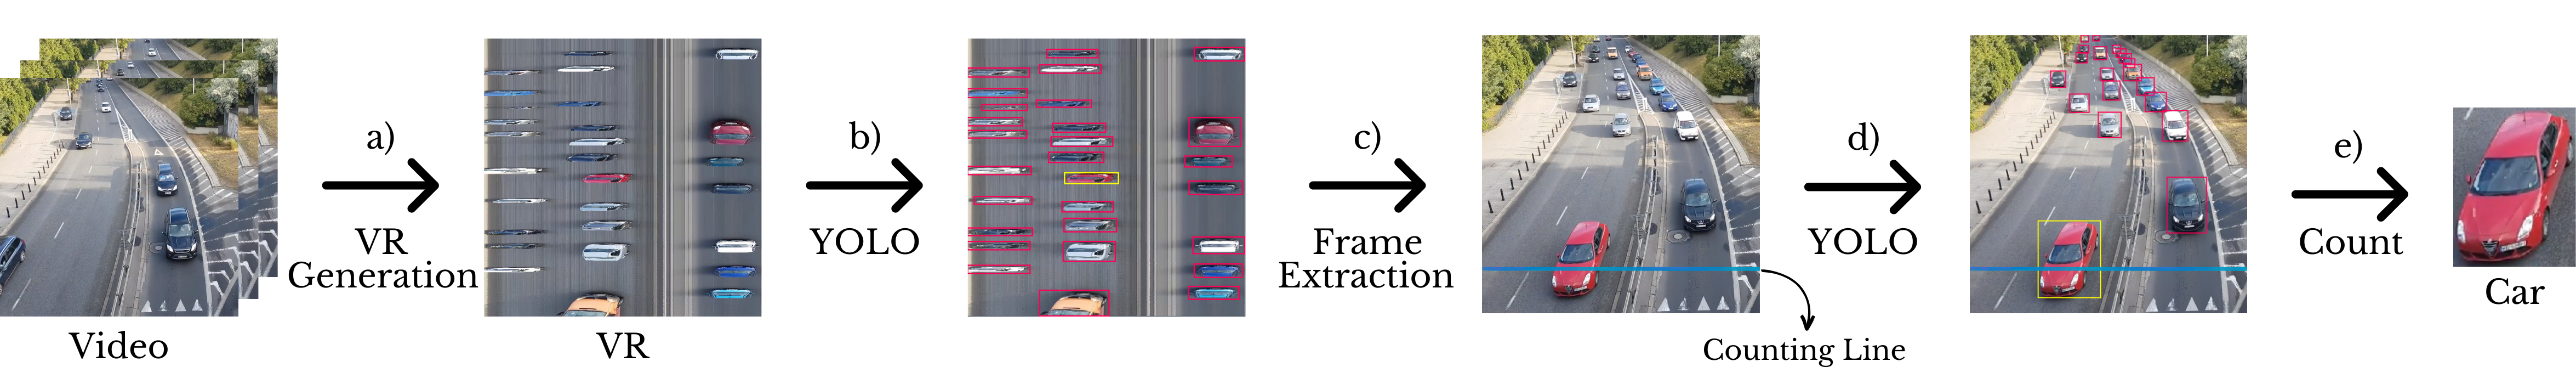
\includegraphics[width=\textwidth]{figs/Method.png}
    \caption{Data flow in the VR–based video counting vehicles.}
    \label{fig:method}
\end{figure*}

%Building upon this premise (\nina{which one?)}, our process follows: a) 
First, in step (a), we create a Visual Rhythm image for segments of $T$ consecutive frames. Assuming a vehicle $i$ intersects the counting line in $T_i$ frames when crossing the counting line, the resultant VR image will contain a mark corresponding to vehicle $i$ with height equal to $T_i$ and width equal to the width of the vehicle. It is important to note, however, that certain marks in the VR image may not correspond to vehicles; for instance, any object crossing the counting line would also produce a corresponding mark. 

In the second step, we employ YOLO to detect each of the marks within the VR image (step (b)). Detecting these marks could be also achieved through background subtraction techniques. However, these methods could fail in handling varying weather conditions, sunlight intensity, and other sources of noise.

Next, for each mark in the VR image, we extract the corresponding frame from the video segment (step (c)). To that end, we know that the $y$ coordinate of the mark's center correspond to the temporal index of the frame when the vehicle's center crossed the counting line. In the diagram of Figure~\ref{fig:method} the extracted frame corresponds to the vehicle highlighted in yellow in the VR image.

After the relevant frame is obtained, we must certify that the mark in question indeed corresponds to a vehicle. Thus, in step (d) we use YOLO to detect all vehicles in the extracted frame and then, for each detected vehicle, we compute the distance between the $x$ coordinates of the vehicle's bounding box and the $x$ coordinates of the mark in the VR image. The vehicle that best matches the size and position of the mark is selected as the one corresponding to the mark. If there are more than one, the one with closest $y$ coordinate is selected as the vehicle corresponding to the mark, and the counting of the vehicle class is updated (step (e)).

%Subsequently, e) we select the vehicle linked to the mark and increase the count according to its class category. This sequence is then repeated for the next $t$ frames of the video until its conclusion. Importantly, the last iteration's duration might be less or equal than $t$.  Moreover, in cases where YOLO misclassifies a mark in previous steps, if no vehicle is in proximity to the counting line, that mark is disregarded and excluded from the counting process.

It is important to note that the above method is applied on sequences of length $T$ in order to keep the VR image size manageable by YOLO. Thus, to process long video sequences, they are partitioned into contiguous and non-overlapping segments of length $T$.
This approach can sometimes lead to situations where the same vehicle appears in the VR images of two consecutive segments. %is represented by two distinct marks in different sequential VRs.
To avoid double counting, we implement a verification process. Specifically, we check if the coordinates of a mark fall along the lower edge of a VR image; if they do, we store these coordinates. As we proceed to create and analyze the subsequent VR, we examine whether any mark appear along the upper edge of the image. 
%and then if the $x$ coordinates of their centers are within the coordinates of the previously stored marks. In such cases, 
If so, and if its $x$ coordinate match the ones stored previously, then we disregard this mark, as it corresponds to the same vehicle in the preceding VR image. This verification process is carried out for each generated VR image. Figure \ref{fig:double-count} shows a visual representation of this situation, where we see that the center coordinates of an mark is within the other mark coordinates. 

\begin{figure}[htp]
    \centering
    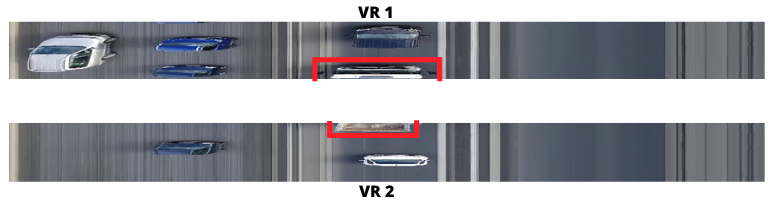
\includegraphics[width=3.25in]{figs/DoubleCounting.png}
    \caption{Vehicle represented by distinct marks in two consecutive VR images.}
    \label{fig:double-count}
\end{figure}

\section{Results and discussion}
To implement the proposed vehicle detection and counting method, we used a computer equipped with a GeForce GTX 1080 Ti running on an Ubuntu operating system. The implementation was carried out using Python, utilizing the Ultralytics and OpenCV libraries.

In this study, we ultilized YOLOv8-small. To enhance its vehicle detection performance, we employed transfer learning by fine-tuning its pre-trained model in a task-specific dataset. This technique was applied to detecting marks and vehicles.

\subsection{Datasets and training}

We use 4 publicly available videos captured from a top-view perspective by a static camera, in diverse locations and scenarios. This highlights the variation in camera angles, the number of lanes for vehicles, and their directions.
To fine-tune YOLO for vehicle detection, we built a dataset consisting of 960 frames randomly selected from these videos, as outlined in Table \ref{tab:dataset}.
%These images were extracted from , the same ones utilized during mark detection training.
We defined 6 vehicle classes: Bus, Car, Motorbike, Pickup, Truck, and Van, and annotated all occurrences of instances of these classes in these selected frames %Each class was meticulously labeled and 
using the Roboflow's framework \cite{roboflow}.

\begin{table}[htp]
\renewcommand{\arraystretch}{1.3}
    \caption{Description of the Dataset's Image Distribution}
    \label{tab:dataset}
    \centering
    \begin{tabular}{|c||c||c|}
        \hline
        Video & Video Length (frames) & \# of Selected Frames\\
        \hline
        1 & 720 & 60\\ %30s
        \hline
        2 & 9180 & 300\\ %306
        \hline
        3 & 20340 & 300\\ %687
        \hline
        4 & 62880 & 300\\ %2096
    \hline
    \end{tabular}
\end{table}



All frame images were resized to a uniform 1280$\times$720 resolution, without any additional preprocessing or augmentation. Refer to Figure \ref{fig:dataset} for frame samples of the dataset.
%from the included dataset locations.

\begin{figure}[htp]
    \centering
    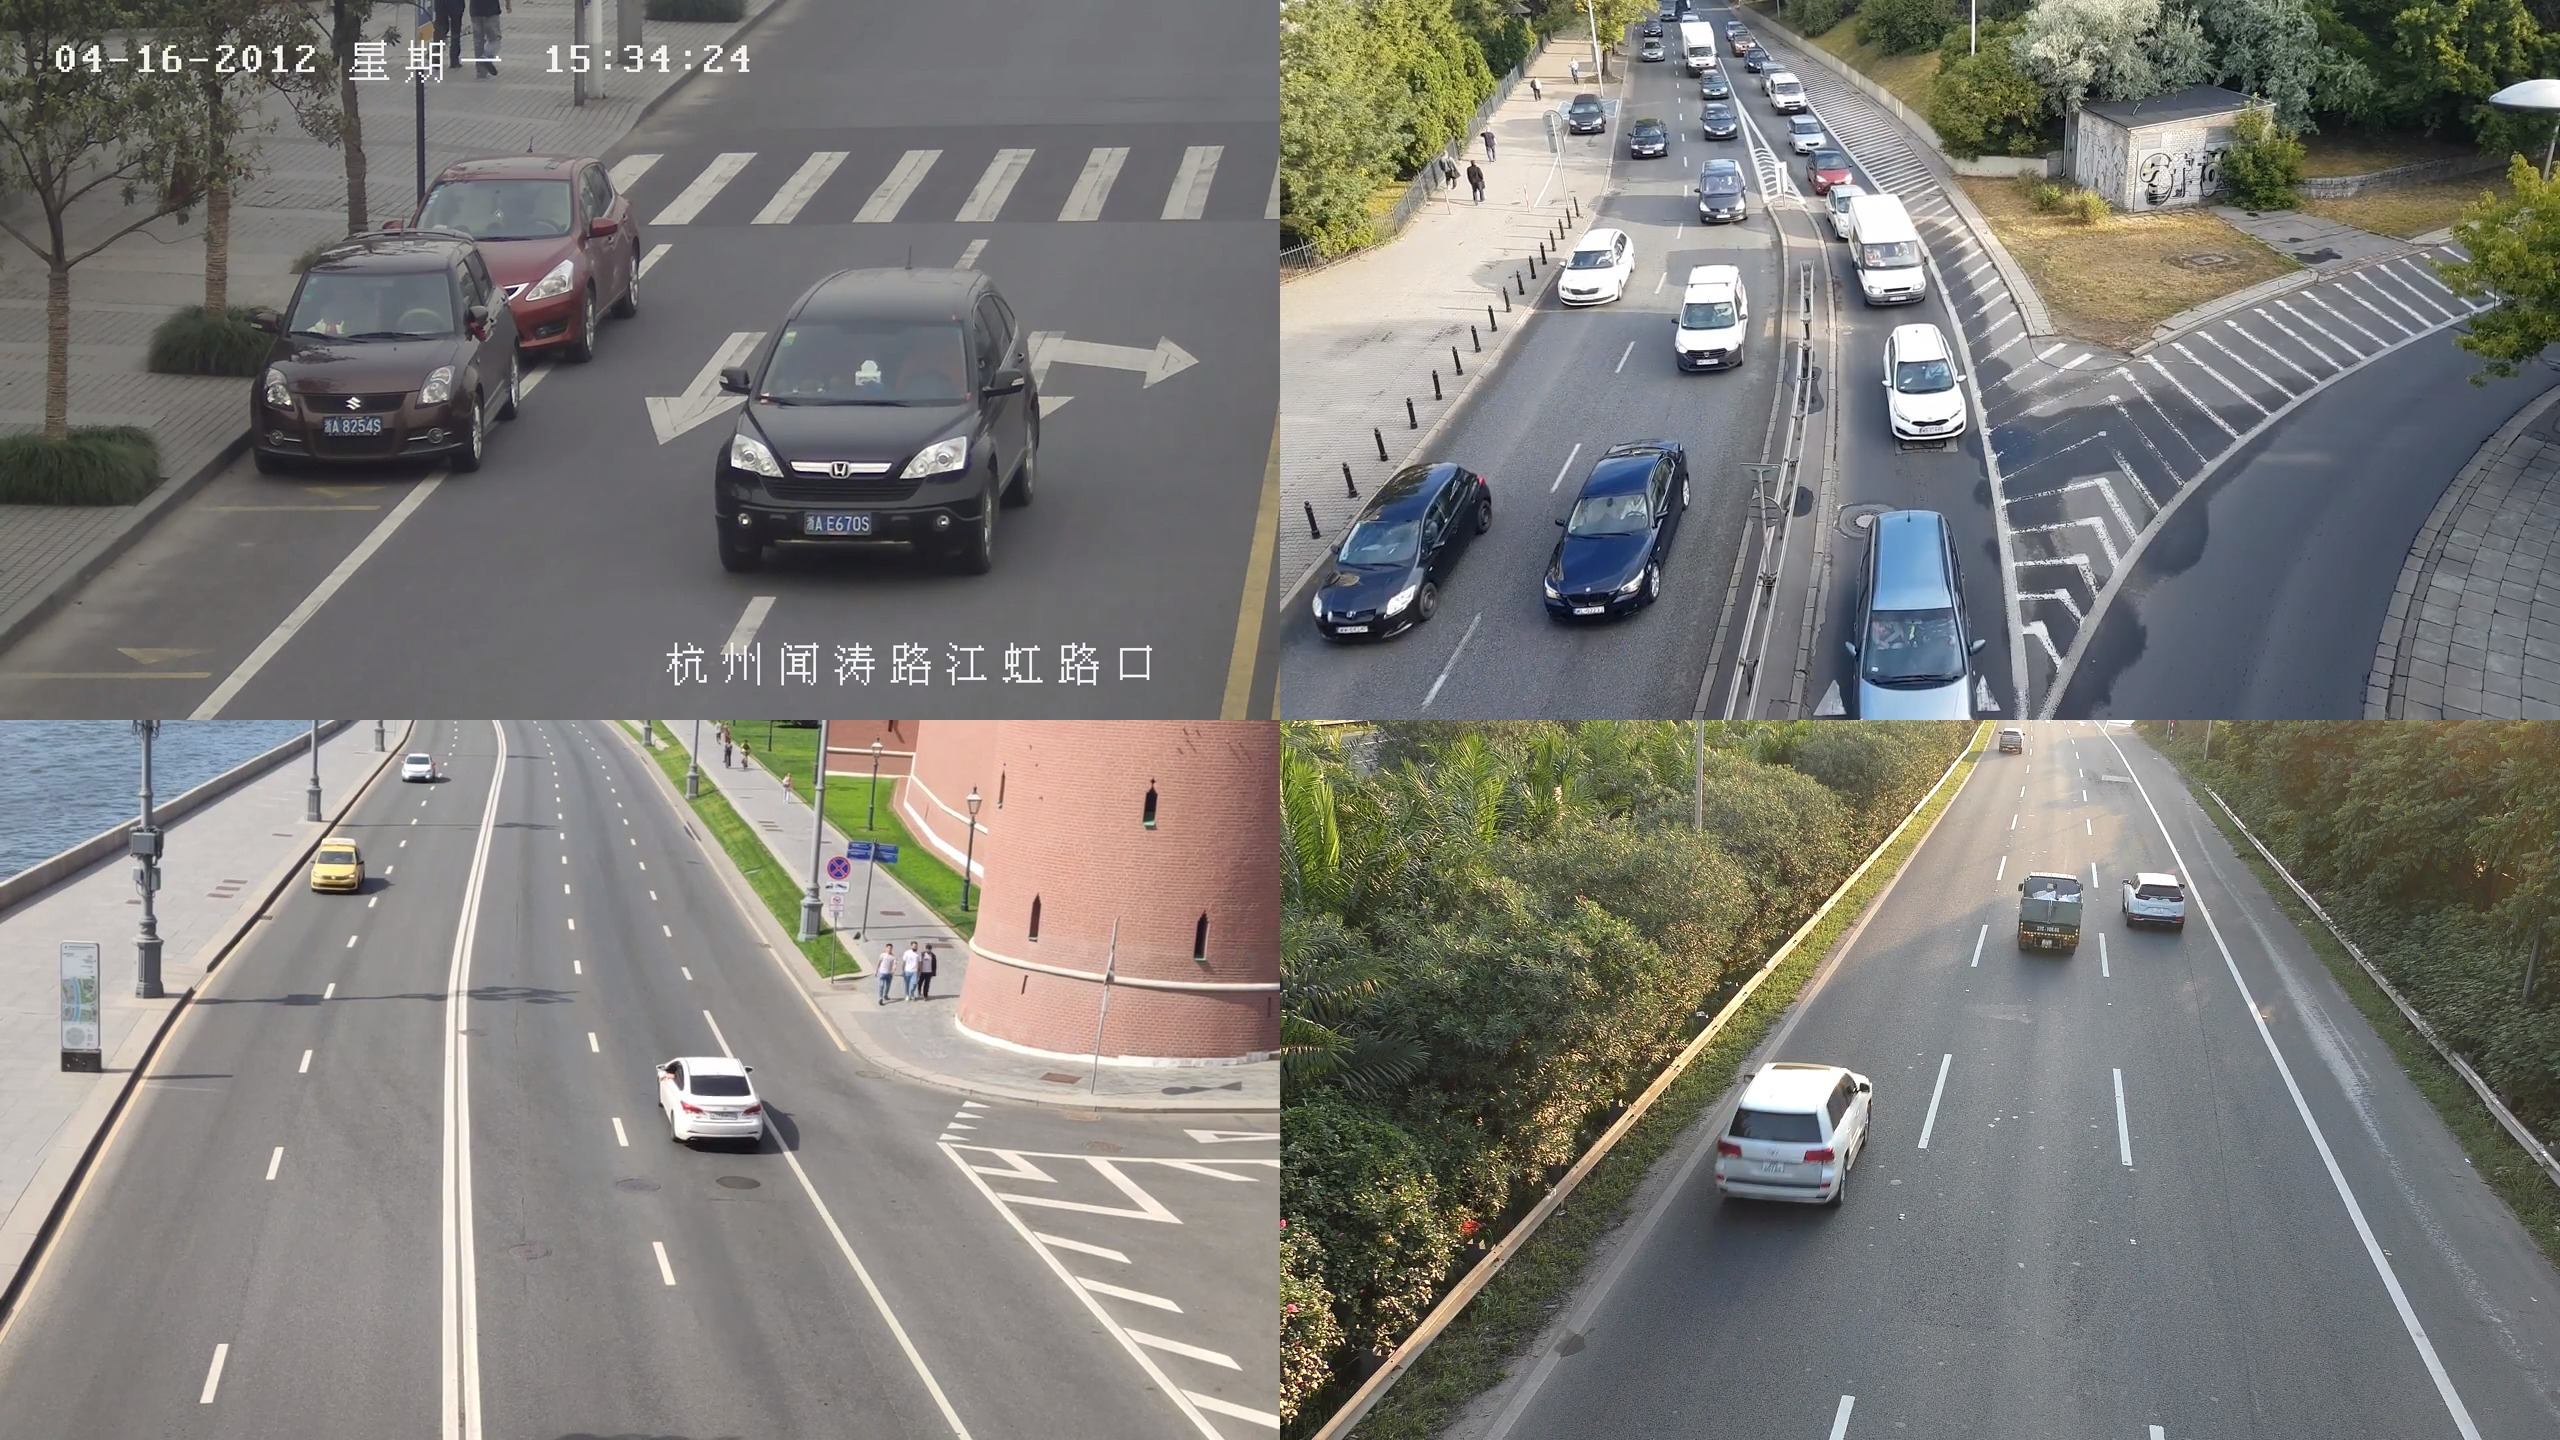
\includegraphics[width=2.5in]{figs/data-merge.jpg}
    \caption{Images samples from the dataset}
    \label{fig:dataset}
\end{figure}

The dataset was partitioned into training, validation, and testing subsets. To that end, from each video, the first 70\% of the selected frames were included in the training set, the next 20\% in the validation set, and the last 10\% to the testing set. We also took care to ensure that a same vehicle is not included in more than one of the sets. 

To train the model for mark detection, we generated 33 VR images corresponding to segments of $T=900$ frames (30 seconds) around the frames in the training and validation sets for vehicle detection described above. The marks have been manually annotated in these VR images. We further augmented our dataset by applying horizontal and vertical flips, along with cropping, resulting in a total of 79 images.

For training, we set up 60 epochs with a batch size of 8 for mark detection, and 100 epochs with a batch size of 64 for vehicle detection, using YOLOv8's standard configuration for other hyperparameters. The mark detection model achieved a final Mean Average Precision (mAP) of 0.99136 at IoU 0.5 and 0.60865 at IoU 0.5:0.95 on the validation set. For vehicle detection, the results were mAP of 0.84274 at IoU 0.5 and 0.69166 at IoU 0.5:0.95, also on the validation set.

\subsection{Results}
In our experiments, we used segments with length $T=900$ frames (30 seconds) to build the VR images, an optimal size for YOLO processing. The counting line was positioned at a height of 120 pixels on the original videos, ensuring coverage of the entire vehicle path. We compare our approach efficiency to Roboflow's frame-by-frame vehicle counting and detection system \cite{roboflow}. This system employs ByteTrack for tracking and supervision for real-time object counting. For both systems, identical environments and model weights were utilized. %Testing images were exclusively sourced from the dataset's test set and weren't part of the training phase. 
Table \ref{tab:test1} shows a comparison of the two methods  on the test segment across various videos, with counting accuracy computed regardless of vehicle class. We did not include the first video due to its short duration.

\begin{table}[htp]
\renewcommand{\arraystretch}{1.3}
    \caption{Counting Accuracy in Each Video}
    \label{tab:test1}
    \centering
    \begin{tabular}{|c||c||c||c||c|}
        \hline
        System & Frame rate & Video 2 & Video 3 & Video 4\\
        \hline
        Visual Rhythm & 186 FPS & 100\% & 98.90\%  & 98.56\% \\
        \hline
        ByteTrack & 56 FPS & 100\% & 99.04\% & 98.48\%\\
    \hline
    \end{tabular}
\end{table}

The results demonstrate that our Visual Rhythm-based method presented an efficiency improvement of approximately three times when compared to the traditional detection and tracking method. This efficiency gain is largely attributed to the elimination of the need for frame-by-frame processing, which significantly contributes to enhancing overall system performance. Moreover, it's worth noting that the generation of VR images, a crucial aspect of our approach, is not overly computationally demanding. More importantly, the gain in efficiency did not impact counting accuracy. We also analyze the results of these approaches when determining the vehicle classes while performing counting. Table \ref{tab:test2} shows our approach's classification accuracy over the test set (four videos). 

\begin{table}[htp]
\renewcommand{\arraystretch}{1.3}
    \caption{Classification Accuracy in Each Video on VR Approach}
    \label{tab:test2}
    \centering
    \begin{tabular}{|c||c||c||c||c||c|}
        \hline
        Car & Bus & Motorbike & Pickup & Truck & Van\\
        \hline
        99.1\% & 86.0\% & 81.6\% & 77.0\% & 96.2\% & 92.9\% \\
    \hline
    \end{tabular}
\end{table}

%These outcomes offer insights into the model's performance in classifying distinct vehicle types. 
Remarkably, the "Car" category exhibits the highest accuracy, with an impressive 99.1\% accuracy rate. However, classifying "Pickup" and "Motorbike" proves comparatively more challenging, with accuracies of 77.0\% and 81.6\%, respectively, which are low. 
%It's crucial to consider that classification errors were calculated for detected and counted vehicles, although misclassified in terms of class. Thus, the lower accuracy in these categories could be attributed to the dataset's limited representation of vehicles from these classes.
We note that the accuracies were computed taking into consideration only the detected and counted vehicles. Classes that exhibit lower accuracies are those less frequent in the dataset.


\section{Conclusion}
The initial hypothesis pointing that the fusion of YOLO with Visual Rhythm for vehicle counting and detection would enhance system performance has been confirmed. Our approach outperforms traditional methods, with a speed-up of approximately 3 times. This show the efficacy of discarding the frame-by-frame processing. Moreover, our approach maintains approximately the same accuracy levels as tracking methods, effectively capturing vehicles through Visual Rhythm but has the disadvantage of not being a real-time application. 

Applying transfer learning to fine-tune YOLO's pre-trained model for task of vehicle detection show satisfactory results in terms of mAP . However, as this metric is calculated across all possible classes, the model's limitations become apparent when analyzing the details presented in Table \ref{tab:test2}. Therefore, there is room for further improvement in the model's performance, particularly by including more examples from classes with low classification accuracy.



% conference papers do not normally have an appendix


% use section* for acknowledgment
\section*{Acknowledgment}

The authors thank support from MCTI (\textit{Ministério da Ciência, Tecnologia e Inovações, Brazil}), law 8.248, PPI-Softex - TIC 13 - 01245.010222/2022-44, \textit{Fundação de Apoio à Universidade de São Paulo} (FUSP), and FAPESP (grant 2015/22308-2).

%The authors whould like to thank \textit{Fundação de Apoio à Universidade de São Paulo} (FUSP) for providing support for this research.




% % An example of a floating figure using the graphicx package.
% % Note that \label must occur AFTER (or within) \caption.
% % For figures, \caption should occur after the \includegraphics.
% % Note that IEEEtran v1.7 and later has special internal code that
% % is designed to preserve the operation of \label within \caption
% % even when the captionsoff option is in effect. However, because
% % of issues like this, it may be the safest practice to put all your
% % \label just after \caption rather than within \caption{}.
% %
% % Reminder: the "draftcls" or "draftclsnofoot", not "draft", class
% % option should be used if it is desired that the figures are to be
% % displayed while in draft mode.
% %

% \begin{figure}[!t]
% \centering
% 
\includegraphics[width=2.5in]{sibgrapi2022.png}
% % where an .eps filename suffix will be assumed under latex, 
% % and a .pdf suffix will be assumed for pdflatex; or what has been declared
% % via \DeclareGraphicsExtensions.
% \caption{SIBGRAPI - Conference on Graphics, Patterns and Images.}
% \label{fig_sim}
% \end{figure}

% % Note that the IEEE typically puts floats only at the top, even when this
% % results in a large percentage of a column being occupied by floats.


% % An example of a double column floating figure using two subfigures.
% % (The subfig.sty package must be loaded for this to work.)
% % The subfigure \label commands are set within each subfloat command,
% % and the \label for the overall figure must come after \caption.
% % \hfil is used as a separator to get equal spacing.
% % Watch out that the combined width of all the subfigures on a 
% % line do not exceed the text width or a line break will occur.
% %
% \begin{figure*}[!t]
% \centering
% \subfloat[Case I]{
\includegraphics[width=2.5in]{figs/sibgrapi2022.png}%
% \label{fig_first_case}}
% \hfil
% \subfloat[Case II]{
\includegraphics[width=2.5in]{figs/sibgrapi2022.png}%
% \label{fig_second_case}}
% \caption{SIBGRAPI - Conference on Graphics, Patterns and Images.}
% \label{fig_sim2}
% \end{figure*}
% %
% % Note that often IEEE papers with subfigures do not employ subfigure
% % captions (using the optional argument to \subfloat[]), but instead will
% % reference/describe all of them (a), (b), etc., within the main caption.
% % Be aware that for subfig.sty to generate the (a), (b), etc., subfigure
% % labels, the optional argument to \subfloat must be present. If a
% % subcaption is not desired, just leave its contents blank,
% % e.g., \subfloat[].


% % An example of a floating table. Note that, for IEEE style tables, the
% % \caption command should come BEFORE the table and, given that table
% % captions serve much like titles, are usually capitalized except for words
% % such as a, an, and, as, at, but, by, for, in, nor, of, on, or, the, to
% % and up, which are usually not capitalized unless they are the first or
% % last word of the caption. Table text will default to \footnotesize as
% % the IEEE normally uses this smaller font for tables.
% % The \label must come after \caption as always.
% %
% \begin{table}[]
% %% increase table row spacing, adjust to taste
% \renewcommand{\arraystretch}{1.3}
% % if using array.sty, it might be a good idea to tweak the value of
% % \extrarowheight as needed to properly center the text within the cells
% \caption{An Example of a Table}
% \label{table_example}
% \centering
% %% Some packages, such as MDW tools, offer better commands for making tables
% %% than the plain LaTeX2e tabular which is used here.
% \begin{tabular}{|c||c|}
% \hline
% One & Two\\
% \hline
% Three & Four\\
% \hline
% \end{tabular}
% \end{table}


% % Note that the IEEE does not put floats in the very first column
% % - or typically anywhere on the first page for that matter. Also,
% % in-text middle ("here") positioning is typically not used, but it
% % is allowed and encouraged for Computer Society conferences (but
% % not Computer Society journals). Most IEEE journals/conferences use
% % top floats exclusively. 
% % Note that, LaTeX2e, unlike IEEE journals/conferences, places
% % footnotes above bottom floats. This can be corrected via the
% % \fnbelowfloat command of the stfloats package.




% % trigger a \newpage just before the given reference
% % number - used to balance the columns on the last page
% % adjust value as needed - may need to be readjusted if
% % the document is modified later
% %\IEEEtriggeratref{8}
% % The "triggered" command can be changed if desired:
% %\IEEEtriggercmd{\enlargethispage{-5in}}

% % references section

% % can use a bibliography generated by BibTeX as a .bbl file
% % BibTeX documentation can be easily obtained at:
% % http://mirror.ctan.org/biblio/bibtex/contrib/doc/
% % The IEEEtran BibTeX style support page is at:
% % http://www.michaelshell.org/tex/ieeetran/bibtex/


























\bibliographystyle{IEEEtran}
% argument is your BibTeX string definitions and bibliography database(s)
\bibliography{example}
%
% <OR> manually copy in the resultant .bbl file
% set second argument of \begin to the number of references
% (used to reserve space for the reference number labels box)
%\begin{thebibliography}{1}
%
%\bibitem{IEEEhowto:kopka}
%H.~Kopka and P.~W. Daly, \emph{A Guide to \LaTeX}, 3rd~ed.\hskip 1em plus
%  0.5em minus 0.4em\relax Harlow, England: Addison-Wesley, 1999.

%\end{thebibliography}




% that's all folks
\end{document}


